\section{Results}
\label{sec:results}

In this section we present the main results of this work, namely the determination
of the photon PDF $\gamma(x,Q^2)$ from a fit to the HERA structure functions
and ATLAS high-mass Drell-Yan cross-sections.
%
In the following we will present results obtained using the
double-differential $\lp m_{ll},y_{ll}\rp$ distributions, though
we have verified that compatible results
are obtained if the $\lp m_{ll},\Delta\eta_{ll}\rp$ ones are fitted
instead.
%
Using the NNLO fit settings discussed in Sect.~\ref{sec:fitsettings}, we find
a $\chi^{2}/N_{\rm dof} = 1.18$,
with a partial $\chi^2/N_{\rm dof} = 1.15$ for the high-mass Drell-yan data.
%
First of all we present our results for the photon PDF, and then the impact
of the DY measurements on the quark and gluon PDF.
%
We will denote as {\tt xFitter\_epHMDY} the results of this work.

In Fig.~\ref{photon_zoom} we show our results
for $\gamma(x,Q^2)$ for $Q^2=10^4$ GeV$^2$,
compared with LUXqed~\cite{Manohar:2016nzj}, HKR~\cite{Harland-Lang:2016apc}
and NNPDF3.0QED.
%
The comparison is restricted to the range $0.05 \le x \le 0.3$ corresponding
to the region where the fitted Drell-Yan measurements have direct kinematic sensitivity
to the photon PDF.
%
For NNPDF3.0QED, we show the 68\% CL uncertainty, while for LUXqed the uncertainty band
is obtained by adding in quadrature all the model variations.

%%%%%%%%%%%%%%%%%%%%%%%%%%%%%%%%%%%%%%%%%%%%%%%%%%%%%%%%
\begin{figure}[h]
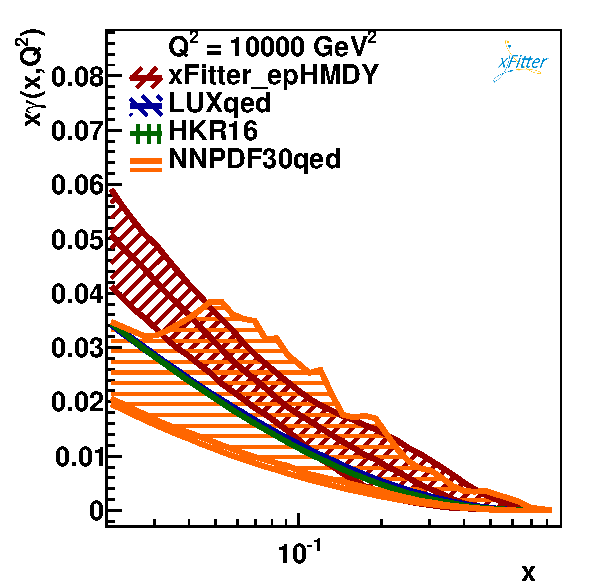
\includegraphics[width=7cm]{figs/photon_comp_10000.pdf} 
\caption{Comparison between $\gamma(x,Q^2)$ at $Q^2=10^4$ GeV$^2$ in the present
  analysis with the corresponding results from NNPDF3.0QED, LUXqed and HKR.}
\label{photon_zoom}
\end{figure}
%%%%%%%%%%%%%%%%%%%%%%%%%%%%%%%%%%%%%%%%%%%%%%%%%%%%%%%%

From the results of Fig.~\ref{photon_zoom} we find that in the region where the HMDY data is
sensitive to the photon PDF, there is good agreement between the four determinations.
%
As compared to NNPDF3.0QED, the PDF uncertainties in the current analysis are reduced, though
they are still not competitive with those of LUXqed.
%
We also note the excellent agreement between the LUXqed and the HKN calculations,
illustrating the commonalities between the two approaches.

Next in Fig.~\ref{photon_zoom_ratio} we show the same comparison of different
results for the photon PDF $x\gamma(x,Q^2)$ now normalized to the central value of {\tt xFitter\_hmDY}.
%
This format allows better to compare the relative compatibility between the various results,
as well as the relative size of the PDF uncertainties in each case.
%
We observe that the experimental uncertainty on {\tt xFitter\_hmDY} is at the $\sim 30\%$ level,
depending on the specific value of $x$, improving over NNPDF3.0QED but still far from the
percent accuracy of the LUXqed calculation.

%%%%%%%%%%%%%%%%%%%%%%%%%%%%%%%%%%%%%%%%%%%%%%%%%%%%%%%%
\begin{figure}[h]
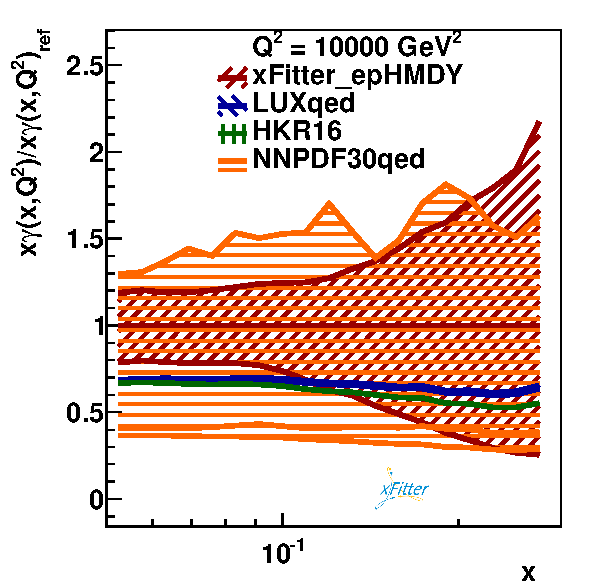
\includegraphics[width=7cm]{figs/photon_comp_10000_ratio.pdf} 
\caption{Same as Fig.\ref{photon_zoom_ratio}, now where results
  are shown normalized to the central value of {\tt xFitter\_hmDY}.
  {\bf update with final result, missing xFitter band.}
  }
\label{photon_zoom_ratio}
\end{figure}
%%%%%%%%%%%%%%%%%%%%%%%%%%%%%%%%%%%%%%%%%%%%%%%%%%%%%%%%

Another interesting question that our analysis allows addressing is what is
the impact of the high-mass Drell-Yan 8 TeV measurements on the quark and gluon
PDFs.
%
For this purpose, and since HERA data alone (which should be used as benchmark for
this comparison) does not have sensitivity to the photon PDF,
we have repeated our fits this time switching off QED effects and thus setting to zero
the photon PDF.
%
This way, we can perform a meaningful comparison between the HERA-only baseline and the
HERA+hmDY fit to gauge the modifications of quark and gluon PDFs.

This comparison is shown in Fig.~\ref{fig:QCDfit} for the up and down antiquarks,
for which the effect of the high-mass
Drell-Yan data is expected to be more marked, and the PDFs are presented
as ratio to the central value of the HERA+hmDY fit.
%
As is apparent from this comparison, the modifications in the medium and large-$x$
antiquarks from the hmDY data are significant for $x\ge 0.01$, though the two fits
agree always at the one-sigma level.
%
Specially for the case of $x\bar{d}$, the improvement in PDF uncertainties
is also marked.

%%%%%%%%%%%%%%%%%%%%%%%%%%%%%%
\begin{figure}[h]
\centering
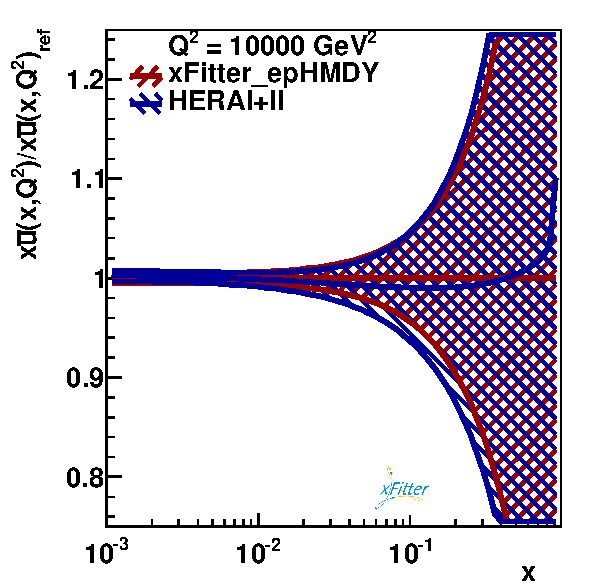
\includegraphics[width=7cm]{figs/q2_10000_pdf_ubar_ratio}
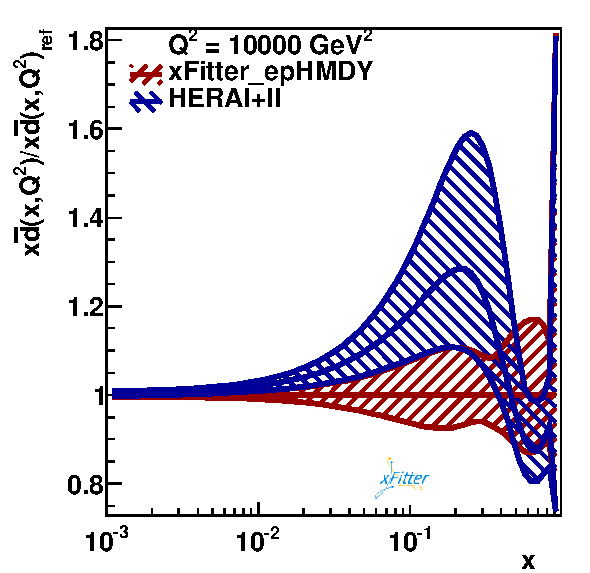
\includegraphics[width=7cm]{figs/q2_10000_pdf_dbar_ratio} 
\caption{The impact of the ATLAS high-mass 8 TeV Drell-Yan measurements
  on the $x\bar{u}$ and $x\bar{d}$ sea quark PDFs at $Q^2=10^4$ GeV$^2$.
  %
  Results are shown normalized to the central value of the HERA+hmDY fit.
}
\label{fig:QCDfit}
\end{figure}
%%%%%%%%%%%%%%%%%%%%%%%%%%%%%%%

After this comparison at the level of PDFs, we move to a comparison between the theoretical
predictions and the high-mass Drell-Yan measurements.
%
First of all, the values of the $\chi^2$ for the HERA structure functions
and for the high-mass DY data for the NNLO fit
are summarized in Table~\ref{tab:chi2fit}.
%
As can be seen, the agreement between data and the NNLO theory
is very good for all the $m_{ll}$ of the 8 TeV Drell-Yan data.
%
For the sum of all the five rapidity bins, we find a $\chi^2=55$
for 48 data points.
%
The quality of the agreement with the HERA inclusive structure functions
is similarly good.
%
In the calculation of the total $\chi^2$, the correlations between the different
$m_{ll}$ bins have been taken into account.

%%%%%%%%%%%%%%%%%%%%%%%%%%%%%%%%%%%%%%%%%%%%
\begin{table}[h]
  \centering
  \begin{tabular}{|c|c|}
    \hline
    Dataset  &   $\chi^2$ \\
    \hline
    \hline
    hmDY  116 GeV $\ge m_{ll} \ge $ 150 GeV  &  9.3/12 \\
    hmDY  150 GeV $\ge m_{ll} \ge $ 200 GeV  &  17/12 \\
    hmDY  200 GeV $\ge m_{ll} \ge $ 300 GeV  &  17/12 \\
    hmDY  300 GeV $\ge m_{ll} \ge $ 500 GeV  &  3.8/6 \\
    hmDY  500 GeV $\ge m_{ll} \ge $ 1500 GeV  &  4.2/6 \\
    \hline
    Correlated $\chi^2$ & 4.98 \\
    Log penalty $\chi^2$  & -0.0004 \\
    \hline
    \hline
    Total  & 55/48 \\
    \hline
    \end{tabular}
  \caption{$\chi^{2}$ for high-mass Drell Yan data for the NNLO fit.
    %
    We show the results for the individual $m_{ll}$ bins
    are well as for the total dataset. {\bf updated
    with HERA numbers}
\label{tab:chi2fit}
  }
\end{table}
%%%%%%%%%%%%%%%%%%%%%%%%%%%%%%%%%%%

Next, in Fig.~\ref{hmDY_2D} we show the
comparison between the ATLAS high-mass Drell Yan data and the NNLO fit predictions
for the  two representative bins of of the $(y_{ll},m_{ll})$ distribution,
  in particular the first and fourth bins.
%
In the lower panel we shows the ratio of theory over data, where the yellow band
corresponds to the correlated systematic uncertainties.
%
The band around the theory prediction corresponds to the total
theory uncertainty from the PDF fit.
%
The shifts due to systematic uncertainties are indicated by a dashed line.

%%%%%%%%%%%%%%%%%%%%%%%%%%%%%%
\begin{figure}[h]
\centering
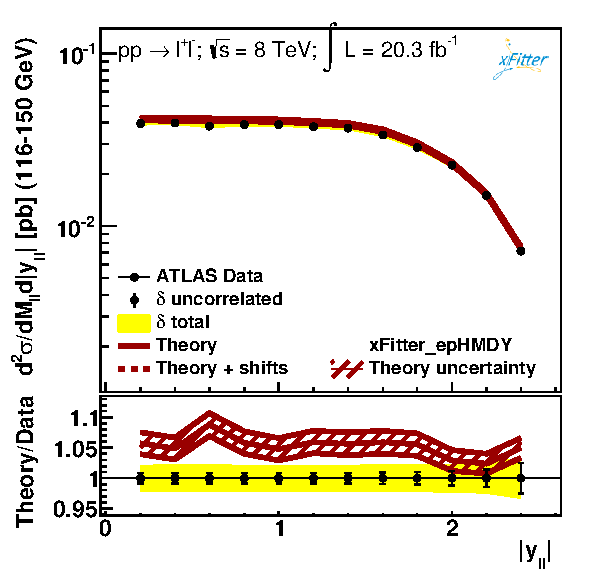
\includegraphics[width=7cm]{figs/data_1.pdf}
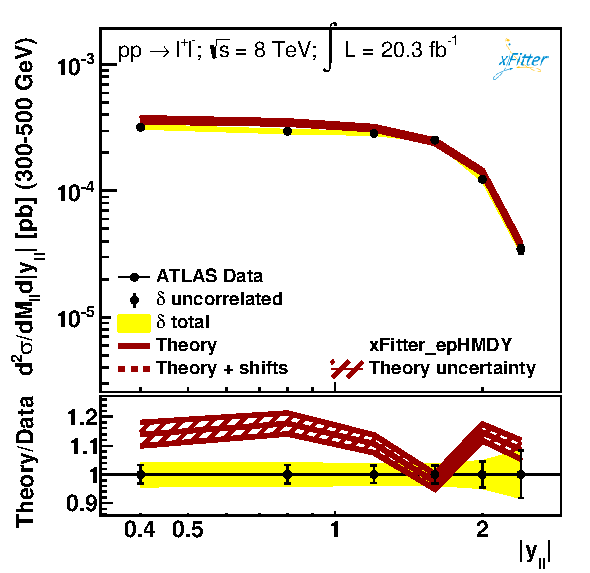
\includegraphics[width=7cm]{figs/data_404-1.pdf} 
\caption{Comparison between the ATLAS high-mass Drell Yan data and the NNLO fit predictions
  for two representative bins of of the $(y_{ll},m_{ll})$ distribution,
  in particular the first and fourth bins.
  %
  The lower panel shows the ratio of theory over data, where the yellow band
  corresponds to the correlated systematic uncertainties.
  %
  The band around the theory prediction corresponds to the total
  theory uncertainty from the PDF fit. {\bf missing shifts? Remove
  luminosity info}
}
\label{hmDY_2D}
\end{figure}
%%%%%%%%%%%%%%%%%%%%%%%%%%%%%%%

As we can see from Fig.~\ref{hmDY_2D}, once the shifts due to experimental systematic
uncertainties have been accounted for, there is a reasonable agreement
between the ATLAS data and the NNLO theory predictions.
%
This agreement is consistent the values of the $\chi^2$ reported in
Table~\ref{tab:chi2fit}, and extends for other $m_{ll}$ bins.
%
We emphasize the high precision of this measurement, with experimental
errors at the few percent level in most of the kinematical range available.

Following this presentation of the main features of this
{\tt xFitter\_hmDY} analysis, now we turn to discuss its stability
and study the impact of a number of model, parametrization,
and procedural uncertainties.

\subsection{Model, parametrization, and procedural uncertainties}

Check the effect of the various variations on the photon PDF, but separately variation per variation,
showing the most important ones, and not stacking the error into a common error band

An important cross-check of the robustness of the estimated uncertainty for the photon
PDF in this analysis is provided by the comparison of the Monte Carlo method
with the Hessian method.
%
In Fig.~\ref{fig:photon_mc_vs_hessian} we show this comparison,
which indicates a reasonable agreement between the two methods.
%
In particular, the central values of the photon obtained with the two fitting
techniques are quite similar to each other.

%%%%%%%%%%%%%%%%%%%%%%%%%%%%%%
\begin{figure}[h]
\centering
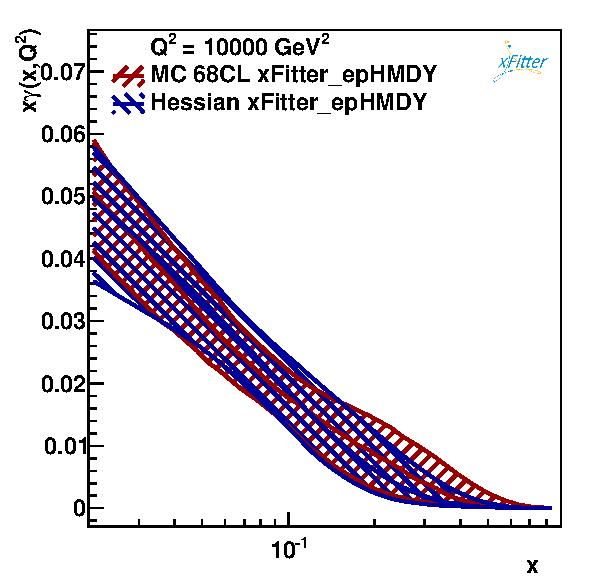
\includegraphics[width=7cm]{figs/photon_mc_vs_hessian} 
\caption{Comparison between $x\gamma(x,Q^2)$ obtained with the
  Monte Carlo method with that from the Hessian method,
  at $Q^2=10^4$ GeV$^2$.
  %
  In both cases the PDF error band corresponds to the 68\% confidence level
  uncertainties.}
\label{fig:photon_mc_vs_hessian}
\end{figure}
%%%%%%%%%%%%%%%%%%%%%%%%%%%%%%%


